\section{Results}
\label{sec:results}

\subsection{The fix restores context integrity without changing base accuracy}

\begin{figure}[t]
\centering
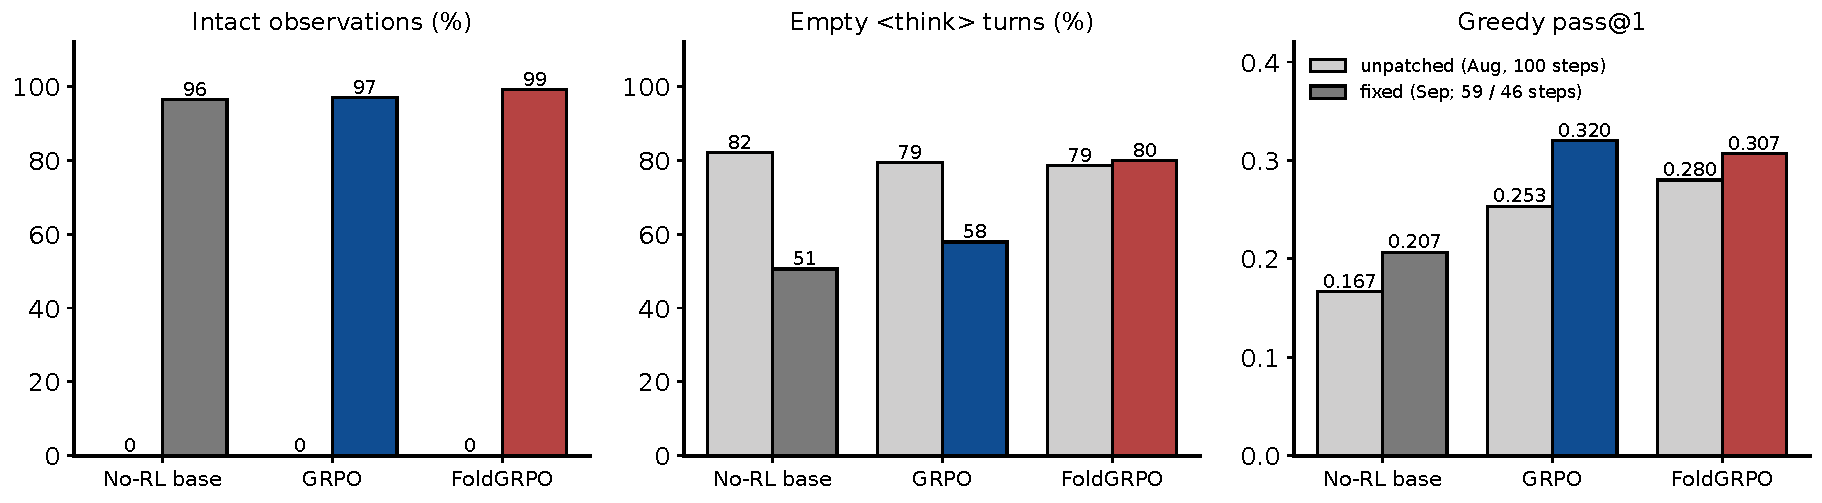
\includegraphics[width=\linewidth]{figures/fig4_bug_contrast.pdf}
\caption{Unpatched versus fixed code, greedy decoding, 150 trajectories per bar. Grey bars are
the earlier study's runs (unpatched code, 100 training steps); colored bars are the post-fix
runs (no-RL base; \grpo{} checkpoint 60, 59 reward-bearing steps; \foldgrpo{} checkpoint 50,
46 steps). Left: share of non-finish tool calls followed by a complete \toolresp{} block; the
remainder after the fix are cut by the 32k-token response limit. Middle: share of assistant
turns whose \think{} block is empty. Right: greedy pass@1 with the same judge; the RL bars are
not budget-matched across code versions and are descriptive only.}
\label{fig:contrast}
\end{figure}

With the fix, 96--99\% of tool calls in every arm are followed by a complete observation block,
against 0\% under the unpatched code (\cref{fig:contrast}, left). On the no-RL base the share
of empty think blocks fell from 82\% to 51\% of turns and the number of main-thread turns per
trajectory fell from 6.9 to 4.5, while greedy pass@1 moved from 0.167 to 0.207 ($\pm 0.065$)
and temperature-1.0 mean@4 from 0.168 to 0.170 ($\pm 0.030$). The fix therefore changed how
the base model behaves but not, within the confidence intervals, how often it is right.

\subsection{Retrained on fixed code, \foldgrpo{} and \grpo{} remain tied}

\begin{table}[t]
\centering
\small
\begin{tabular}{lcccc}
\toprule
Checkpoint & Reward-bearing steps & Greedy pass@1 & $T{=}1.0$ mean@4 & $T{=}1.0$ best@4 \\
\midrule
No-RL base & 0 & 0.207 ($\pm$0.065) & 0.170 ($\pm$0.030) & 0.298 \\
\grpo{} 40 & 40 & 0.307 ($\pm$0.074) & 0.308 ($\pm$0.037) & 0.411 \\
\grpo{} 50 & 50 & 0.300 ($\pm$0.073) & 0.323 ($\pm$0.037) & 0.443 \\
\grpo{} 60 & 59 & 0.320 ($\pm$0.075) & \textbf{0.342} ($\pm$0.038) & 0.439 \\
\foldgrpo{} 40 & 40 & \textbf{0.353} ($\pm$0.076) & 0.320 ($\pm$0.037) & 0.460 \\
\foldgrpo{} 50 & 46 & 0.307 ($\pm$0.074) & 0.335 ($\pm$0.038) & \textbf{0.466} \\
\bottomrule
\end{tabular}
\caption{Pass@1 on the 150-item \bcplus{} test split, graded by \judgemodel{} through the
training-stack validation path. Greedy: $n{=}150$; $T{=}1.0$: 600 graded trajectories,
mean@4 and best-of-4. Intervals are binomial 95\% CIs; the $T{=}1.0$ intervals treat the four
samples per item as independent and are optimistic. Bold marks the best value per column.}
\label{tab:main}
\end{table}

\begin{figure}[t]
\centering
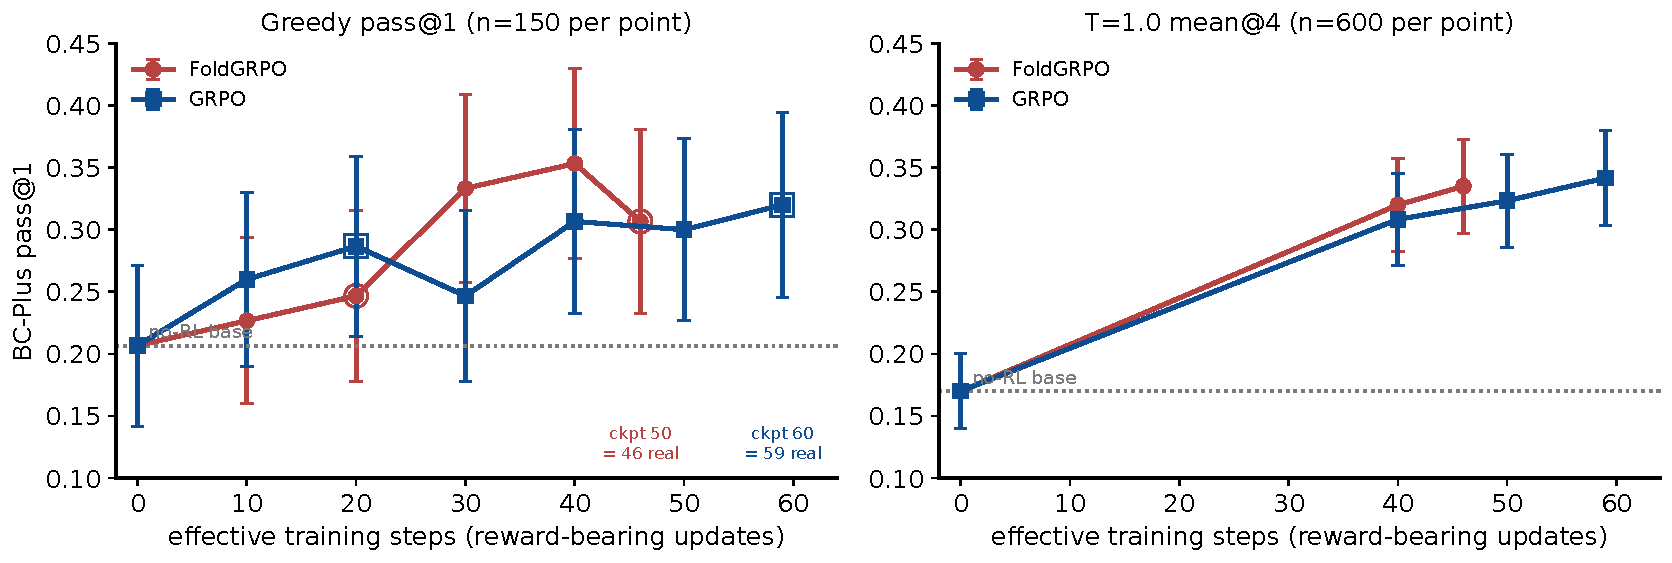
\includegraphics[width=\linewidth]{figures/fig1_scores_vs_step.pdf}
\caption{Validation score against reward-bearing training steps for both arms. Left: greedy
pass@1 ($n{=}150$ per point); right: $T{=}1.0$ mean@4 (600 per point). Error bars are 95\%
binomial CIs; the dotted line is the fixed no-RL base. Hollow rings mark val-only
re-evaluations of the uploaded checkpoint, used where the in-process validation ran inside an
infrastructure gap. \foldgrpo{} checkpoint 50 contains 46 reward-bearing updates and \grpo{}
checkpoint 60 contains 59 (\cref{sec:budget}); all earlier checkpoints are fully real.}
\label{fig:scores}
\end{figure}

Both arms left the base within 10 steps and kept improving to the end of their effective
budgets (\cref{tab:main}, \cref{fig:scores}). At the decisive temperature-1.0 tier, mean@4
rose from 0.170 to 0.335 for \foldgrpo{} after 46 steps and to 0.342 for \grpo{} after 59, a
gain of 16--17 points that exceeds the paired interval several times over. The RL gain is
larger than the 10--11 points of the earlier study, which trained 100 steps on the unpatched
code.

The two objectives did not separate. At the step-matched checkpoint 40, where both arms are
fully reward-bearing, \foldgrpo{} led \grpo{} by 4.6 points at greedy decoding (0.353 versus
0.307) and by 1.2 points at temperature 1.0 (0.320 versus 0.308, best@4 0.460 versus 0.411);
both differences are inside the respective intervals. At the last uncontaminated checkpoints
the order reversed at temperature 1.0 (0.335 versus 0.342) while \foldgrpo{}'s greedy score
fell from 0.353 to 0.307. Greedy decoding at $n{=}150$ cannot rank checkpoints whose true
scores differ by a few points, and the temperature-1.0 tier shows no difference to rank.
\foldgrpo{} reached \grpo{}'s final temperature-1.0 score with 13 fewer reward-bearing
updates, which is consistent with a mild sample-efficiency advantage but does not establish one.

\begin{figure}[t]
\centering

\includegraphics[width=\linewidth]{figures/fig2_training_curves.pdf}
\caption{Training dynamics from the per-step trainer logs: batch-mean trajectory reward over
256 rollouts, train overlong rate, and mean response length. Solid segments had a live reward
server; crosses mark steps hit by a scheduled reclamation of the search-and-judge node before
the final loss (scores zeroed or rollouts cut short); shaded and dotted segments follow the
final loss on September 12, after which \foldgrpo{} steps have gradient norm exactly zero and
\grpo{} steps carry only exact-match rewards (\cref{sec:budget}). The \foldgrpo{} train overlong
rate is zero by construction of its reward accounting and is not comparable with \grpo{}'s;
the evaluation overlong rate in \cref{tab:behavior} is.}
\label{fig:training}
\end{figure}

Training reward rose from 0.085 to 0.170 (\foldgrpo{}, first five versus last ten
reward-bearing steps) and from 0.093 to 0.153 (\grpo{}), with policy entropy between 0.04 and
0.27 nats in both arms and no collapse (\cref{fig:training}). Mean response length doubled from
about 10k to about 20k tokens in both arms, and step time grew accordingly from 13 to 65
minutes (\foldgrpo{}) and 48 minutes (\grpo{}).
